\documentclass[a4paper,11pt]{scrartcl}
\usepackage[utf8]{inputenc}
\usepackage[english]{babel}
\usepackage{tikz}
\usepackage{amsmath}
\usepackage{mathtools}
\usepackage{dsfont}
\usepackage{float}


\DeclarePairedDelimiter\abs{\lvert}{\rvert}
\DeclarePairedDelimiter\norm{\lVert}{\rVert}


\title{Numerical Simulation of Fluids}

\author{Jan H\"onig \\ \texttt{jan.hoenig@fau.de}}


\date{Winter term 2015 - R\"ude}


\usetikzlibrary{calc,trees,positioning,arrows,chains,shapes.geometric,%
    decorations.pathreplacing,decorations.pathmorphing,shapes,%
    matrix,shapes.symbols}

\tikzset{
>=stealth',
  punktchain/.style={
    rectangle, 
    rounded corners, 
     fill=black!10,
    draw=black, very thick,
    text width=10em, 
    minimum height=3em, 
    text centered, 
    on chain},
  line/.style={draw, thick, <-},
  element/.style={
    tape,
    top color=white,
    bottom color=blue!50!black!60!,
    minimum width=8em,
    draw=blue!40!black!90, very thick,
    text width=10em, 
    minimum height=3.5em, 
    text centered, 
    on chain},
  every join/.style={->, thick,shorten >=1pt},
  decoration={brace},
  tuborg/.style={decorate},
  tubnode/.style={midway, right=2pt},
}
\begin{document}

\maketitle

\vfill

This summary was written by a student, correctness of the content can not be guaranteed. The script mostly consists of lecture notes. The lecture itself is strongly oriented on the book Numerical Simulation in Fluid Dynamics and thus all formulas or pictures have the same numbering as in the book, in order to facilitate any further research.


\newpage
\tableofcontents
\newpage

\section{Introduction}
How to uncover laws of nature?
\begin{itemize}
	\item practical $\rightarrow$ observation of experiments
	\item theoretical $\rightarrow$ relations ship between mathematical quantities
	\item[!] often experiments impossible (nuclear reactor, oil sill, too long, too short, where to measure) and mathematical equations too complex (only simplified models)
	\item[$\rightarrow$] numerical simulation: combines both approaches, see Figure~\ref{fig:simproc}
\end{itemize}

\subsection{Simulation Procedure}

\begin{figure}[H]
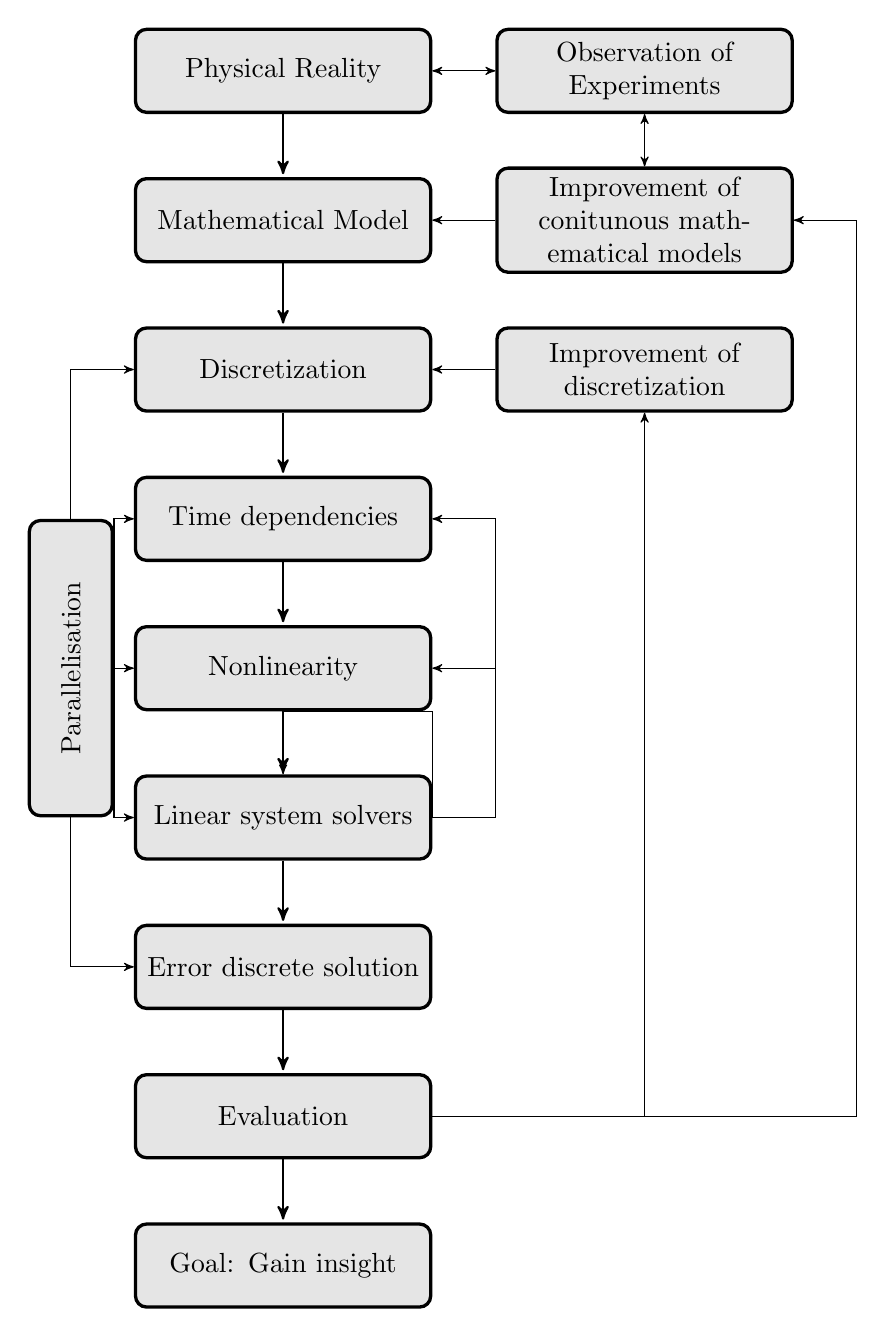
\begin{tikzpicture}
  [node distance=.8cm,
  start chain=going below,]
    \node[punktchain, join] (phys) {Physical Reality};
    \node[punktchain, join] (math)      {Mathematical Model};
    \node[punktchain, join] (discr)      {Discretization};
    \node[punktchain, join] (time-dept) {Time dependencies};
    \node[punktchain, join] (nonlin) {Nonlinearity};
  	\node[punktchain, join] (lin) {Linear system solvers};
    \node[punktchain, join] (error) {Error discrete solution};
    \node[punktchain, join] (eval) {Evaluation};
    \node[punktchain, join] (goal) {Goal: Gain insight};

    \node [punktchain, right=of phys] (obs) {Observation of Experiments};
	\node [punktchain, right=of math] (improvec) {Improvement of conitunous mathematical models};
    \node [punktchain, right=of discr] (improved) {Improvement of discretization};
    \node [punktchain, left=of time-dept, rotate=90] (parallel) {Parallelisation};
	
	\coordinate[right=of lin] (lin-right);
	\coordinate[right,above=of lin] (lin-top);
    
    \coordinate[right=of nonlin] (nonlin-right);

	\draw[->] (lin.east) |- (lin-top) -| (lin.north);
	\draw[->] (lin.east) -| (nonlin-right) -- (nonlin.east);
	\draw[->] (lin.east) -| (nonlin-right) |- (time-dept.east);

    \draw[->] (eval.east) -| (improved.south);
     
    \draw[->] (parallel.east) |- (discr.west);
    \draw[->] (parallel.south) |- (nonlin.west);
    \draw[->] (parallel.south) |- (time-dept.west);
    \draw[->] (parallel.south) |- (lin.west);
    \draw[->] (parallel.west) |- (error.west);

	\coordinate[right=of improvec] (improvec-coord);
	\draw[->] (eval.east) -| (improvec-coord) -- (improvec);

   	\draw[<->] (obs) -- (improvec);
    \draw[<->] (obs) -- (phys);   		   
 		   
  	\draw[->] (improvec) -- (math);   
   	\draw[->] (improved) -- (discr);
	

  \end{tikzpicture}
  
  \renewcommand{\thefigure}{1.1}
  \caption{Typical procedure in numerical simulation}
  \label{fig:simproc}
\end{figure}

  
\subsection{Fluids and Flows}

Fluids $\left\{
\begin{tabular}{c}
    gas \\
    liquids
\end{tabular}
\right\}$ are substances that cannot resist shear forces. \\
Examples: Water, Coffee, Air, Stream, Waterfall\\
Engineering: Flow around a car, flow pipeline. Often the iteration of a flow with a solid body, fluid sturcture interaction, multi-phase flows (gas $\leftrightarrow$ liquid).

\paragraph{Properties of Fluids}
\begin{itemize}
	\item Viscosity
	\begin{itemize}
		\item Frictional forces that act on the fluid
		\item[$\rightarrow$] Without external forces the fluid will come to a rest. The higher the viscosity, the faster it comes to a rest.
		\item Highly viscous (honey) $\rightarrow$ frictional forces are strong
		\item In gases viscous forces small $\rightarrow$ sometimes neglected
		\item[$\rightarrow$] "inviscid flow" in gas dynamics $\rightarrow$ Euler equation
	\end{itemize}
	\item Inertia
	\begin{itemize}
		\item[$\rightarrow$] Reynolds number : $\frac{\text{inertia}}{\text{viscosicty}}$
		\item[$\rightarrow$] high $\rightarrow$ turbulence; low $\rightarrow$ laminar
	\end{itemize}
	\item Compressibility
	\begin{itemize}
		\item Gases at high velocities are compressible
		\item Liquids are nearly incompressible
		\item[$\rightarrow$] Important if temperature changes
	\end{itemize}
\end{itemize}

Boundary layer theory
\begin{itemize}
	\item[$\rightarrow$] close to boundary, velocity is slow $\rightarrow$ viscous forces $\sim$ inertia forces
	\item[$\rightarrow$] away from boundaries, velocity high $\rightarrow$ viscous forces $<$ inertia forces
\end{itemize}
%TODO pictures (2)

\subsection{Numerical Fluid Simulation}
Our goal: Simulate unsteady, incompressible, laminar flow, Navier-Stokes equations\\
\paragraph{History}
\begin{itemize}
	\item[$\rightarrow$] Dictated by compute power
	\item precursors: Crank-Nickelson '47
	\item real start: Harlow-Fromm '65
	\item in this course: "marker-and-cell" (MAC) method, Harlow-Welch '65
	\begin{itemize}
		\item simple
		\item flexible
		\item efficient
	\end{itemize}
	\item Alternatives: Finite elements, Finite Volumes, SIMPLE, QUICK
\end{itemize}

\section{Mathematical description of flows}
\begin{itemize}
	\item laminar
	\item viscious
	\item incompressible
\end{itemize}
\subsection{Mathematical Model}
\begin{itemize}
	\item Spatial domain: $\Omega \subset  \mathds{R}^2$ or $\Omega \subset  \mathds{R}^3$
	\item Time $t \in [0, t_{end}]$
	\item Fluid is characteristic by:
	\begin{itemize}
		\item Velocity: $\vec{u} : \Omega \times [0, t_{end}] \rightarrow \mathds{R}^2$
		\item Pressure: $p : \Omega \times [0, t_{end}] \rightarrow \mathds{R}$
		\item Density: $ \varrho : \Omega \times [0, t_{end}] \rightarrow \mathds{R}$
		\item[$\rightarrow$] Incompressible: $\varrho(\vec{x},t) = \varrho_\infty = \text{const}$
	\end{itemize}
\end{itemize}
Governing equations, a system of partial differential equations (Navier-Stokes eq.) are (~\ref{fig:momentum} and ~\ref{fig:cont-eq}):

\begin{figure}[H]
	\centering
	\[\frac{\delta \vec{u}}{\delta t} + ( \vec{u} \cdot \text{grad}) \vec{u} + \text{grad} p = \frac{1}{Re} \Delta \vec{u} + \vec{g}\]
	\renewcommand{\thefigure}{2.1.a}
    \caption{Momentum Equation}
	\label{fig:momentum}
\end{figure}
\begin{figure}[H]
	\centering
	\[\text{div} \vec{u} = 0\]
	\renewcommand{\thefigure}{2.1.b}
    \caption{Continuity Equation}
	\label{fig:cont-eq}
\end{figure}

\begin{itemize}
	\item grad $p := (\frac{\delta p}{\delta x},\frac{\delta p}{\delta y})^T$
	\item div $\vec{u} := \frac{\delta u}{\delta x} + \frac{\delta v}{\delta y}$
	\item $\vec{u} \text{ grad} := \left( \begin{pmatrix}
		u \\
		v
	\end{pmatrix}
	\cdot \begin{pmatrix}
		\frac{\delta}{\delta x} \\
		\frac{\delta}{\delta y}
	\end{pmatrix}\right)
	= (u \cdot \frac{\delta}{\delta x} + v \frac{\delta}{\delta y})$
	\item $(\vec{u} \text{ grad} ) \vec{u} = \left( u \cdot \frac{\delta}{\delta x} + v \frac{\delta}{\delta y}\begin{pmatrix}
		u \\
		v
	\end{pmatrix}\right) = \begin{pmatrix}
		u \frac{\delta u}{\delta x} & v \frac{\delta u}{\delta y}\\
		u \frac{\delta v}{\delta x} & v \frac{\delta v}{\delta y}
	\end{pmatrix}$
	\item $Re \in \mathds{R} \Rightarrow$ Reynolds number
	\item $\vec{g} \in \mathds{R} \Rightarrow$ Body forces (i.e. gravity)
	\item $\vec{x} = \begin{pmatrix}
	x\\
	y
	\end{pmatrix}; \vec{u} = \begin{pmatrix}
	u\\
	v
	\end{pmatrix}; \vec{p} = \begin{pmatrix}
	p_x \\
	p_y
	\end{pmatrix}$
\end{itemize}

\begin{figure}[H]
	\centering
	\[ \frac{\delta u}{\delta t} + \frac{\delta p}{\delta x} = \frac{1}{Re} \left( \frac{\delta^2 u}{\delta x^2} + \frac{\delta^2 u}{\delta y^2}\right) - \frac{\delta (u^2)}{\delta x} - \frac{\delta (uv)}{\delta y} + g_x\]
    \renewcommand{\thefigure}{2.2a}
	\caption{Momentum Equation u}
	\label{fig:momentuma}
\end{figure}
\begin{figure}[H]
	\centering
	\[ \frac{\delta v}{\delta t} + \frac{\delta p}{\delta y} = \frac{1}{Re} \left( \frac{\delta^2 v}{\delta x^2} + \frac{\delta^2 v}{\delta y^2}\right) - \frac{\delta (uv)}{\delta x} - \frac{\delta (v^2)}{\delta y} + g_y\]
    \renewcommand{\thefigure}{2.2b}
	\caption{Momentum Equation v}
	\label{fig:momentumb}
\end{figure}
\begin{figure}[H]
	\centering
	\[ \frac{\delta u}{\delta x} + \frac{\delta v}{\delta y}\]
    \renewcommand{\thefigure}{2.2c}
	\caption{Continuity Equation}
	\label{fig:cont}
\end{figure}


At $t = 0$ initial conditions $u(t=0, x,y) = u_0(x,y)$ and $v(t=0,x,y) = v_0(x,y)$ \textbf{must} satisfy \ref{fig:cont}.


For all times along the boundary of the domain $\Omega$ we have \textbf{boundary condition}: "initial-boundary value problem".

To formulate the boundary condition, we introduce $\varphi_n$ velocity component nominal to the boundary and $\varphi_t$ velocity component tangential to the boundary. When the boundary is aligned with the coordinate direction: 


$\left.\begin{matrix}
\varphi_n = u\\
\varphi_t = v
\end{matrix} \right\rbrace$ vertical boundary $\left\lbrace \frac{\delta \varphi_n}{\delta n} = \frac{\delta u}{\delta x},\frac{\delta \varphi_t}{\delta n} = \frac{\delta v}{\delta x} \right\rbrace$

$\left.\begin{matrix}
\varphi_n = v\\
\varphi_t = u
\end{matrix} \right\rbrace$ vertical boundary $\left\lbrace \frac{\delta \varphi_n}{\delta n} = \frac{\delta v}{\delta y},\frac{\delta \varphi_t}{\delta n} = \frac{\delta u}{\delta y} \right\rbrace$


The following types of boundary conditions occur:
\begin{enumerate}
	\item \textit{No-slip condition}: No fluid penetrates the boundary and the fluid is at rest there
	\[ \varphi_n(x,y) = 0, \varphi_t(x,y)=0\]
	\item \textit{Free-slip condition}: No fluid penetrates the boundary. There are no frictional losses at the boundary.
	\[ \varphi_n (x,y)= 0, \frac{\delta \varphi_t(x,y)}{\delta n} = 0 \]
	$\rightarrow$ useful along alined line of symmetry
	\item \textit{Inflow condition}: Both velocity components are given
	\[ \varphi_n(x,y) = \varphi_n^0, \varphi_t(x,y) = \varphi_t^0\]
	\item \textit{Outflow condition}: Neither velocity component changes in the direction normal to the boundary
	\[ \frac{\delta \varphi_n(x,y)}{\delta n} = 0, \frac{\delta \varphi_t(x,y)}{\delta n} = 0\]
	\item \textit{Periodic boundary condition}: For problems which are periodic with a certain period of "a" in on of the coordinate directions (e.g. the flow over modulating surface), computation can be restricted to one period. Velocities and pressure must coincide at the endpoints at the interval. Periodicity in x-direction $\left.\begin{matrix}
	x = 0\\
	x=a
	\end{matrix}\right\rbrace$ boundary
	\[\varphi_n (0, y) = \varphi_n(a,y)\]
	\[ \varphi_t(0,y) = \varphi_t(a,y)\]
	\[ p (0, y) = p(a,y)\]
	
\end{enumerate}

If the velocity components (rather then the derivatives) are given along the entire boundary, then
\[ \int_\Gamma \begin{pmatrix}
u
v
\end{pmatrix} \cdot \vec{n} ds = 0\]
in the Navier-Stoke equation the pressure is only determined up to a constant.


\section{Numerical Discretization of the NS equations}
\begin{itemize}
	\item[$\rightarrow$] Replace \textbf{derivatives} by \textbf{finite differences}
	\item[!] Must be done the right way. Oscillations in pressure otherwise
\end{itemize}


\subsection{Discretization}

\subsubsection{Simple discretization formulas}

\paragraph{Discretization in One Dimension}
Consider an interval $\Omega = [0,a] \subset \mathds{R}$ on which a different equation must be solved, $i_{max}$ sub-intervals of equal size $\delta x = \frac{a}{i_{max}}$ yielding a grid $x_i = i \delta x$
\begin{figure}[H]
	\centering
	\[ \frac{\delta u}{\delta x} = \lim\limits_{\delta x \rightarrow 0} \frac{u(x + \delta x) - u(x)}{\delta x}\]
    \renewcommand{\thefigure}{3.1}
	\caption{Definition of derivative}
	\label{fig:deriv-def}
\end{figure}

\begin{figure}[H]
	\centering
	\[ \left[\frac{d u}{d x}\right]^r_i = \frac{u(x_{i+1}) - u(x_i)}{\delta x}\]
    \renewcommand{\thefigure}{3.2}
	\caption{Forward difference}
	\label{fig:deriv-forward}
\end{figure}

\begin{figure}[H]
	\centering
	\[ \left[\frac{d u}{d x}\right]^l_i = \frac{u(x_i) - u(x_{i+1})}{\delta x}\]
    \renewcommand{\thefigure}{3.3}
	\caption{Backward difference}
	\label{fig:deriv-backward}
\end{figure}

\begin{figure}[H]
	\centering
	\[ \left[\frac{d u}{d x}\right]^c_i = \frac{u(x_{i+1}) - u(x_{i-1})}{2 \delta x}\]
    \renewcommand{\thefigure}{3.4}
	\caption{Central difference}
	\label{fig:deriv-central}
\end{figure}

\begin{itemize}
	\item Accuracy of forward \& backward difference is $O(\delta x)$
	\item Accuracy of central difference is $O(\delta x)^2$
\end{itemize}

\begin{figure}[H]
	\centering
	\[ \left[\frac{d u}{d x}\right] = \frac{1}{\delta x}\left(\left[\frac{d u}{d x}\right]^c_{i+\frac{1}{2}} - \left[\frac{d u}{d x}\right]^c_{i-\frac{1}{2}}\right) = \frac{u(x_{i+1}) - 2u(x_i) + u(x_{i-1})}{(\delta x)^2}  \]
    \renewcommand{\thefigure}{3.5}
	\caption{Second derivative}
	\label{fig:deriv-def2}
\end{figure}


With Figures~\ref{fig:deriv-def} and~\ref{fig:deriv-def2} all necessary discretization of derivatives is provided. However in some case this discretization results into unphysical oscillations.

Consider e.g. a second-order ordinary differential equation (ODE)~\ref{fig:ode} with Dirichlet boundary condition $u(0) = u_0, u(a) = u_{imax}$.
\begin{figure}[H]
	\centering
	\[ -\frac{d^2 u }{dx^2} + k \frac{du}{dx} = f \text{ in } \Omega \]
	\renewcommand{\thefigure}{3.6}
	\caption{Ordinary differential equation of second order}
	\label{fig:ode}
\end{figure}

We can replace the derivatives with the appropriate difference quotients from above~\ref{fig:deriv-def},~\ref{fig:deriv-def2} to obtain \ref{fig:disc-ode} with unknowns $u_i$ approximating $u(x_i)$.

\begin{figure}[H]
	\centering
	\[ -\frac{-u_{i+1} + 2u_i - u_{i-1}}{(\delta x)^2} + \frac{k}{2 \delta x} (u_{i+1} -u_{i-1}) = f(x_i)\]
	\renewcommand{\thefigure}{3.7}
	\caption{Discretization of ordinary differential equation of second order}
	\label{fig:disc-ode}
\end{figure}

In matrix-vector-notation this can be written as $Au = f$, where 

%TODO matrix, vector, func, representation (3.8)
\[
A = ()  u = ()   f = ()
\]

Take a very simple example case. Assume $k >> 1$ (is large), $f(x) = 0$, $\delta x = 1$, $u(0) = e^{-3k} \approx 0$, $u(3) = 0$.

True solution: $u(x) = e^{k(x-3)} \qquad u_0 = e^{-3k} \approx 0 \qquad u_3 = 1$
\[\left.\begin{matrix}
	-u_0 + 2u_1 -u_2  + k(u_2 -u_0) =0\\
	-u_1 + 2u_2 - u_3 + k(u_3-u_1) = 0
	\end{matrix}\right\rbrace \xRightarrow{k >> 1}\begin{matrix}
	u_2 = u_0\\
	u_3 = u_1
	\end{matrix} \]
%TODO pictures

With central differences, oscillations will start to occur when $\delta x > \frac{2}{\abs{k}}$ $\rightarrow$ unstable discretization.

For strongly convective terms, either $\delta x$ is very small, or we use an "upwind discretization". Consider situation from above, with backward differences:

\[\left.\begin{matrix}
	-u_0 + 2u_1 -u_2  + k(u_1 -u_0) =0\\
	-u_1 + 2u_2 - u_3 + k(u_2-u_1) = 0
	\end{matrix}\right\rbrace \xRightarrow{k >> 1}\begin{matrix}
	u_1 = u_0\\
	u_2 = u_1
	\end{matrix} \]

For $k >> 1 \Rightarrow$ backward difference, $k << -1 \Rightarrow$ forward difference.
In general we can use ~\ref{fig:disc-upwind}. This is always stable, but only $O(\delta x)$ accurate. Possible compromise: the weight average between central and upwind discretization \ref{fig:weighted-average} with properly chosen parameter $\gamma = [0,1]$.
\begin{figure}[H]
	\centering
	\[ \left[\frac{d u}{d x}\right]^{du}_i = \frac{ (1+\epsilon) (u_i - u_{i-1} + (1 - \epsilon) (u_{i+1} - u_i)}{ 2 \delta x} \text{ with } \epsilon = \text{sign}(k) \]
	\renewcommand{\thefigure}{3.9}
	\caption{General "upwind" difference}
	\label{fig:disc-upwind}
\end{figure}

\begin{figure}[H]
	\centering
	\[ \gamma \cdot \text{ upwind difference } + (1-\gamma) \cdot \text{ central difference} \]
	\renewcommand{\thefigure}{3.10}
	\caption{Wighted average between central and upwind difference}
	\label{fig:weighted-average}
\end{figure}

Alternatively: "donor-cell-scheme" for the discretization of $\frac{d(ku)}{dx}$:
\begin{figure}[h]
	\centering
	\[ \left[\frac{d(k u)}{d x}\right]^{dc}_i = \frac{ k_r u_r - k_l u_l}{ \delta x} \text{ where } u_r = \begin{cases}
	u_i & k_r > 0\\
	u_{i+1} & k_r < 0
\end{cases} ; u_l = \begin{cases}
u_{i-1} & k_l > 0\\
u_{i} & k_l < 0
\end{cases} \]
	\renewcommand{\thefigure}{3.11}
	\caption{Discretization with the donor-cell scheme}
	\label{fig:dcs-method}
\end{figure}
%TODO line


The formula~\ref{fig:dcs-method} can be rewritten in the form~\ref{fig:dcs-method-rewritten}. With this representation there is no need fore case distinctions. Thus the sign of k denotes the flow direction, these scheme always selects the value which lies in the upstream direction. An averaging of central and donor-cell differences, similar to ~\ref{fig:weighted-average} is another option.
\begin{figure}[H]
	\centering
	\[ \left[\frac{d(k u)}{d x}\right]^{dc}_i = \frac{1}{2 \delta x} \left[ (k_r - \abs{k_r}) u_{i+1} + (k_r + \abs{k_r}-k_l +\abs{k_l}) u_i  + (-k_l -\abs{k_l})u_{i-1} \right] \]
	\renewcommand{\thefigure}{3.12}
	\caption{Rewritten form of the discretization with the donor-cell scheme}
	\label{fig:dcs-method-rewritten}
\end{figure}

\paragraph{Discretization in Two Dimensions}
Initially $\Omega = [0,a] \times [0,b] \subset \mathds{R}^2$
\[i_{max} : \text{cells in x-Direction} \qquad j_{max} : \text{cells in y-Direction}\]
\[\delta x  = \frac{a}{i_{max}} \qquad \delta y = \frac{b}{j_{max}}\]
\[\text{grid} x_{i,j} = (i \delta x, j \delta y), i = 0, \dots, i_{max}, j = 0, \dots, j_{max} \]
$\rightarrow$ Grid with equal sized cells, with intersection points of the grid lines.

\begin{figure}[H]
	\centering
	\[ [\Delta u]_{ij} = \frac{u(x_{i+1,j}) - 2u(x_{i,j}) + u(x_{i-1,j})}{(\delta x)^2} + \frac{u(x_{i,j+1}) - 2u(x_{i,j}) + u(x_{i,j-1})}{(\delta y)^2}\]
	\renewcommand{\thefigure}{3.13}
	\caption{Discretization at the grid point $x_{i,j}$}
	\label{fig:dcs-method}
\end{figure}

After discretizing Poisson's equation ~\ref{fig:pe-dirich} with Dirichlet boundary conditions, we obtain  a system of $(i_{max}-1)(j_{max})$ equations ~\ref{fig:sys-of-eq} where $u_{i,j}$ approximates $u(x_{i,j})$.
\begin{figure}[H]
	\centering
	\[ \Delta u = f \text{ in } \Omega, \qquad u = g \text{ on } \delta\Omega\]
	\renewcommand{\thefigure}{3.14}
	\caption{Poisson's equation with Dirichlet boundary condition}
	\label{fig:pe-dirich}
\end{figure}

\begin{figure}[H]
	\centering
	\[ \frac{1}{(\delta x)^2} (u_{i+1,j} - 2u_{i,j} + u_{i-1,j}) + \frac{1}{(\delta y)^2} (u_{i,j+1} - 2u_{i,j} + u_{i,j-1}) = f(x_{i,j}) \text{ for } \begin{cases}
	i = 1, \dots, i_{max}-1 \\
	j = 1, \dots, j_{max}-1
\end{cases} \]
	\renewcommand{\thefigure}{3.15}
	\caption{Linear system of equations}
	\label{fig:sys-of-eq}
\end{figure}


Boundary conditions can be incorporated by setting $u_{i,j} = g(x_{i,j})$ for $i \in \lbrace 0, i_{max} \rbrace$ or $j \in \lbrace 0,j_{max} \rbrace$. If the PDE contains 1st-order derivatives, it may be necessary to discretize them by techniques introduced in 1D using upwind or donor-cell discretization.

\subsubsection{Discretization of the NS equation}
\paragraph{Treatment of the Spatial Derivatives}
We will use a staggered grid, i.e. the unknowns are not located at the same grid points. Positions are shifted by $0.5 \cdot \delta x$ and/or $0.5 \cdot \delta y$.
\begin{itemize}
	\item pressure $p$ in cell centers
	\item horizontal velocity $u$ in midpoints of vertical cell edges
	\item vertical velocity $v$ in midpoints of horizontal cell edges
\end{itemize}
%TODO picture


Problems occur on the boundary: need to introduce a "boundary strip".

Staggered grid $\Rightarrow$ no pressure oscillations\\
Consider problem discretized with all unknowns $u,v,p$ on same grid points, then for trivial boundary conditions $(u = 0, v =0, g_x = g_y = 0)$ a solution would be $u = 0, v = 0, p = \text{const}$ on a non staggered grid $u_{i,j} = 0, v_{i,j} = 0$ but $p = \begin{cases}
p1 & i+j \text{even}\\
p2 & i+j \text{odd}
\end{cases}$

Discretization on a staggered grid: Continuity equation (~\ref{fig:cont}) will be discretized at center of each cell $i = 1, \dots, i_{max}; j = 1, \dots, j_{max}$ by replacing $\frac{\delta u}{\delta x}$ and $\frac{\delta v}{\delta y}$ by central differences ~\ref{fig:dif-cen-stag}.

\begin{figure}[H]
	\centering
	\[ \left[ \frac{\delta u}{\delta x}\right]_{i,j} = \frac{u_{i,j} - u_{i-1,j}}{\delta x}; \qquad  \left[ \frac{\delta v}{\delta y}\right]_{i,j} = \frac{v_{i,j} - v_{i,j-1}}{\delta y} \]
	\renewcommand{\thefigure}{3.16}
	\caption{Central differences on staggered grid}
	\label{fig:dif-cen-stag}
\end{figure}

Momentum equation (\ref{fig:momentuma}) discretized at vertical edge midpoints (where u is)

Momentum equation (\ref{fig:momentumb}) discretized at horizontal edge midpoints (where v is)

Second derivatives $\frac{\delta^2 u}{\delta x^2}, \frac{\delta^2 u}{\delta y^2}, \frac{\delta^2 v}{\delta x^2}, \frac{\delta^2 v}{\delta y^2}$ diffusive terms, can be replaced by formula according to ~\ref{fig:deriv-def2}.

Spatial derivative of pressure: central difference with half the mesh width

%TODO sind die dinger im nenner in quadrat???
Difficulty: Discretization $\frac{\delta(u^2)}{\delta x}, \frac{\delta(uv)}{\delta y}, \frac{\delta(uv)}{\delta x}, \frac{\delta(v^2)}{\delta y}$

%TODO picture
At the "x"-points we need approximations of $u \cdot v \rightarrow$ use averages!

\begin{figure}[H]
	\centering
	\[ \left[ \frac{\delta (uv)}{\delta y}\right]_{i,j} = \frac{1}{\delta y}\left[ \left( \frac{v_{i,j} + v_{i,j+1}}{2} \cdot \frac{u_{i,j} + u_{i,j+1}}{2} \right) - \left( \frac{v_{i,j-1} + v_{i+1, j-1}}{2} \cdot \frac{u_{i,j-1} + u_{i,j}}{2}\right) \right] \]
	\renewcommand{\thefigure}{3.17}
	\caption{Discretization with averages}
	\label{fig:disc-spec}
\end{figure}

Similar: $\frac{\delta(u^2)}{\delta x}$ central difference with $\frac{\delta x}{2}$ at "+"-points.

\begin{figure}[H]
	\centering
	\[ \left[ \frac{\delta (u)^2}{\delta x}\right]_{i,j} = \frac{1}{\delta x}\left[ \left( \frac{u_{i,j} + u_{i+1,j}}{2}\right)^2 - \left( \frac{u_{i-1,j} + u_{i, j}}{2}\right)^2 \right] \]
	\renewcommand{\thefigure}{3.18}
	\caption{Discretization with averages}
	\label{fig:disc-spec}
\end{figure}

Because convective terms may be dominant for large u and v, it is necessary to mix central differences with the donor-cell scheme. As in \ref{fig:dcs-method-rewritten} we set:
\[ k_r = \frac{u_{i,j} + u_{i+1,j}}{2} \qquad k_l = \frac{u_{i-1,j} + u_{i,j}}{2} \text{ for } \frac{delta(u^2)}{\delta x}\]
\[ k_r = \frac{v_{i,j} + v_{i+1,j}}{2} \qquad k_l = \frac{v_{i,j-1} + v_{i+1,j-1}}{2} \text{ for } \frac{\delta(uv)}{\delta v}\]
Analogous for $\frac{\delta(uv)}{\delta x}$ and $\frac{\delta(v^2)}{\delta y}$. In total we get in equation \ref{fig:momentuma} for u at the midpoint of the \textbf{right edge} of cell, for all $i,j = \begin{cases}
i = 1, \dots, i_{max-1} \\
j = 1, \dots, j_{max-1}
\end{cases}$

\begin{figure}[H]
	\centering
	\begin{align*}
	 	\left[ \frac{\delta(u^2)}{\delta x}\right]_{i,j} =& \frac{1}{\delta x}\left( \left(\frac{u_{i,j} + u_{i+1,j}}{2} \right)^2 - \left(\frac{u_{i-1,j} + u_{i,j}}{2}\right)^2 \right) \\ &+ \gamma\frac{1}{\delta x} \left( \frac{\abs{u_{i,j} +u_{i+1,j}}}{2} \frac{(u_{i,j} - u_{i+1,j})}{2} - \frac{\abs{u_{i-1,j} + u_{i,j}}}{2} \frac{(u_{i-1,j} - u_{i,j})}{2} \right) \\		
	 	\left[ \frac{\delta(uv)}{\delta y}\right]_{i,j} =& \frac{1}{\delta y} \left( \frac{(v_{i,j} + v_{i+1,j})}{2} \frac{(u_{i,j} + u_{i,j+1})}{2} - \frac{(v_{i,j-1} + v_{i+1,j-1})}{2} \frac{(u_{i,j-1} + u_{i,j})}{2} \right) \\ &+ \gamma \frac{1}{\delta y}  \left( \frac{\abs{v_{i,j} + v_{i+1,j}}}{2} \frac{(u_{i,j} - u_{i+1,j})}{2} - \frac{\abs{v_{i,j-1} + v_{i+1,j-1}}}{2} \frac{(u_{i,j-1} - u_{i,j})}{2} \right) \\
	 	\left[ \frac{\delta^2 u}{\delta x^2}\right]_{i,j} =& \frac{u_{i+1, j} - 2u_{i,j} + u_{i-1,j}}{(\delta x)^2} \\
	 	\left[ \frac{\delta^2 u}{\delta y^2}\right]_{i,j} =& \frac{u_{i, j+1} - 2u_{i,j}  +u_{i,j-1}}{(\delta y)^2} \\
	 	\left[ \frac{\delta p}{\delta x}\right]_{i,j} =& \frac{p_{i+1,j} - p_{i,j}}{\delta x}
	\end{align*}
	
	\renewcommand{\thefigure}{3.19a}
	\caption{Discretization for momentum equation of u~\ref{fig:momentuma}}
	\label{fig:disc-moma}
\end{figure}


In \ref{fig:momentumb} for v at midpoint of the \textbf{upper edge} of a cell, for all $i,j = \begin{cases}
i = 1, \dots, i_{max-1} \\
j = 1, \dots, j_{max-1}
\end{cases}$

\begin{figure}[H]
	\centering
	\begin{align*}
		 	\left[ \frac{\delta(uv)}{\delta x}\right]_{i,j} =& \frac{1}{\delta x} \left( \frac{(u_{i,j} + u_{i,j+1})}{2} \frac{(v_{i,j} + v_{i+1,j})}{2} - \frac{(u_{i-1,j} + u_{i-1,j+1})}{2} \frac{(v_{i-1,j} + v_{i,j}}{2} \right) \\ &+ \gamma \frac{1}{\delta x}  \left( \frac{\abs{u_{i,j} + u_{i,j+1}}}{2} \frac{(v_{i,j} - v_{i+1,j})}{2} - \frac{\abs{u_{i-1,j} + u_{i-1,j+1}}}{2} \frac{(v_{i-1,j} - v_{i,j})}{2} \right) \\
	 	\left[ \frac{\delta(v^2)}{\delta y}\right]_{i,j} =& \frac{1}{\delta y}\left( \left(\frac{v_{i,j} + v_{i,j+1}}{2} \right)^2 - \left(\frac{v_{i,j-1} + v_{i,j}}{2}\right)^2 \right) \\ &+ \gamma\frac{1}{\delta y} \left( \frac{\abs{v_{i,j} +v_{i,j+1}}}{2} \frac{(v_{i,j} - v_{i,j+1})}{2} - \frac{\abs{v_{i,j-1} + v_{i,j}}}{2} \frac{(v_{i,j-1} - v_{i,j})}{2} \right) \\		
	 	\left[ \frac{\delta^2 v}{\delta x^2}\right]_{i,j} =& \frac{v_{i+1, j} - 2v_{i,j} + v_{i-1,j}}{(\delta x)^2} \\
	 	\left[ \frac{\delta^2 v}{\delta y^2}\right]_{i,j} =& \frac{v_{i, j+1} - 2v_{i,j}  +v_{i,j-1}}{(\delta y)^2} \\
	 	\left[ \frac{\delta p}{\delta y}\right]_{i,j} =& \frac{p_{i,j+1} - p_{i,j}}{\delta x}
	\end{align*}
	
	\renewcommand{\thefigure}{3.19b}
	\caption{Discretization for momentum equation of u~\ref{fig:momentumb}}
	\label{fig:disc-momb}
\end{figure}

The parameter $\gamma: 0 \leq \gamma \leq 1$ should be chosen such that:
\begin{figure}[H]
	\centering
	\[ \gamma \geq \max_{i,j} \left( \abs{\frac{u_{i,j} \delta t}{\delta x}}, abs{\frac{v_{i,j} \delta t}{\delta y}}\right) \]
	\renewcommand{\thefigure}{3.20}
	\caption{Hirt et al., 1975}
	\label{fig:gamma}
\end{figure}


\paragraph{Boundary Values for the Discrete Equations}

\ref{fig:disc-moma} for \ref{fig:momentuma} for $u$ involves $u$-values for $i = 1, \dots, i_{max-1}, \left\{
\begin{tabular}{c}
    u-values on boundary \\
    u-values outside boundary
\end{tabular}
\right\} \text{ for }  j = 1, j = j_{max}$

\ref{fig:disc-momb} for \ref{fig:momentumb} for $v$ involves $v$-values for $j = 1, \dots, j_{max-1}, \left\{
\begin{tabular}{c}
    v-values on boundary \\
    v-values outside boundary
\end{tabular}
\right\} \text{ for }  i = 1, i = i_{max}$

In total: \begin{tabular}{cc}
on boundary & $\begin{cases}
u_{0,j}, u_{i_{max},j} \text{ for } j = 1, \dots, j_{max}\\ 
v_{i,0}, v_{i,j_{max}} \text{ for } i = 1, \dots, i_{max} 
\end{cases}$ \\
outside boundary & $\begin{cases}
u_{i,0}, u_{i,j_{max+1}} \text{ for } i = 1 , \dots, i_{max} \\ 
v_{0,j}, v_{i_{max+1},j} \text{ for } j = 1, \dots, j_{max} 
\end{cases}$ 
\end{tabular}

%TODO picture

\begin{enumerate}
	\item No-slip boundary condition: continuous velocities must vanish on the boundary ( or be the same velocity as the wall)
For values directly on the boundary, set
\begin{figure}[H]
	\centering
	\[ u_{0,j} = 0, \qquad u_{i_{max},j} = 0, \qquad j = 1,\dots,j_{max} \]
	\[ v_{i,0} = 0, \qquad v_{i,j_{max}} = 0, \qquad i = 1,\dots,i_{max} \]
	\renewcommand{\thefigure}{3.21}
	\caption{Discretization of the No-slip condition}
	\label{fig:disc-nosplipa}
\end{figure}

\begin{figure}[H]
	\centering
	\[ v_r = \frac{v_u + v_i}{2} = 0 \Rightarrow v_a = -v_i\]
	\renewcommand{\thefigure}{3.22}
	\caption{Discretization of the No-slip condition}
	\label{fig:disc-nosplipb}
\end{figure}

This leads to:
%TODO this figure and checko following
\begin{figure}[H]
	\centering
	\[ v_r = \frac{v_u + v_i}{2} = 0 \Rightarrow v_a = -v_i\]
	\renewcommand{\thefigure}{3.23}
	\caption{Discretization of the No-slip condition}
	\label{fig:disc-nosplipc}
\end{figure}

	\item Free-slip
\begin{figure}[H]
	\centering
	\[ u_{0,j} = 0, \qquad u_{i_{max},j} = 0, \qquad j = 1,\dots,j_{max} \]
	\[ v_{i,0} = 0, \qquad v_{i,j_{max}} = 0, \qquad i = 1,\dots,i_{max} \]
	\renewcommand{\thefigure}{3.24}
	\caption{Discretization of the No-slip condition}
	\label{fig:disc-freesplipa}
\end{figure}
%TODO picture

Because the normal derivative $\delta v/ \delta x$ has to be $0 \Rightarrow v_a = v_i$ Further boundary conditions:
\begin{figure}[H]
	\centering
	\[ v_{0,j} = v_{1,j}, \qquad v_{i_{max},j} = v_{i_{max+1}, j}, \qquad j = 1,\dots,j_{max} \]
	\[ u_{i,0} = u_{i,1}, \qquad u_{i,j_{max}} = u_{i,j_{max+1}}, \qquad i = 1,\dots,i_{max} \]
	\renewcommand{\thefigure}{3.25}
	\caption{Discretization of the No-slip condition}
	\label{fig:disc-freesplipb}
\end{figure}
	
	
	\item Outflow boundary condition
Normal derivative of both velocity components set to 0
\begin{figure}[H]
	\centering
	%TODO make 2 times matrix
	\[ u_{0,j} = u_{1,j}, \qquad u_{i_{max},j} = u_{i_{max+1}, j}, \qquad j = 1,\dots,j_{max} \]
	\[ v_{0,j} = v_{1,j}, \qquad v_{i_{max+1},j} = v_{i_{max}, j}, \qquad j = 1,\dots,j_{max} \]
	\[ u_{i,0} = u_{i,1}, \qquad u_{i,j_{max+1}} = u_{i,j_{max}}, \qquad i = 1,\dots,i_{max} \]
	\[ v_{i,0} = v_{i,1}, \qquad v_{i,j_{max}} = v_{i,j_{max+1}}, \qquad i = 1,\dots,i_{max} \]
	\renewcommand{\thefigure}{3.26}
	\caption{Discretization of the Overflow condition}
	\label{fig:disc-outflow}
\end{figure}


	\item Inflow conditions: Velocity explicitly tangential velocity components by averaging simillar to \ref{fig:disc-nosplipb}
	\item Periodic boundary conditions, e.g. periodic in x direction

\begin{figure}[H]
	\centering
	\[ u_{0,j} = u_{i_{max-1},j}, \qquad u_{i_{max},j} = u_{1,j}, \qquad p_{i,j} = p_{i_{max},j} \]
	\[ v_{0,j} = v_{i_{max-1},j}, \qquad v_{1,j} = v_{i_{max},j}, \qquad v_{i_{max+1},j} = v_{2,j}\]
	\renewcommand{\thefigure}{3.27}
	\caption{Discretization of the Periodic boundary condition}
	\label{fig:disc-freesplipb}
\end{figure}
there, different from continuos domain, we have an overlap of one cell width. Periodic in y works analogously.


\end{enumerate}
\paragraph{Discretization of the time derivative}
%TODO bla


\subsection{The Algorithm}

\subsubsection{The time-stepping loop}

%TODO gehen essen



%TODO on notes



%TODO Should be 3.4 and 3.4.1
\subsection{Treatment of general Domains}

\subsubsection{Introduction of obstacle domains}
\begin{itemize}
	\item flow domain $\Omega$ embeded into rectangle $G$, smallest possible size, grid for $G$ as in Sect 3.1 %TODO reference on section
	\item cells of $G$ are divided into
	\begin{itemize}
		\item fluid cells (completly or mostly filled with fluid)
		\item obstacle cells (completly or mostly filled with obstacle)
	\end{itemize}
	\item edges between fluid and obstacle cells $\rightarrow$ \textbf{boundary edges}
	\item solve only in fluid cells
	\item cells $(i,j), i \in \{0, i_{max+1}\}; j \in \{0,j_{max+1}\}$
	(artificial boundary strip) are also treated as obstacle cells
	\item obstacle cells which share an edge with at least one fluid cell are called boundary cells
	\item Fluid cells that are adjacent to the obstacle cells: Compute F,G according to (3.36) (3.37)%TODO ref
	$\Rightarrow$ Need: 
	\begin{itemize}
		\item nomal velocity on the boundary edge
		\item tangential velocity components on edges between boundary cells
	\end{itemize}
	\item[$\Rightarrow$] F,G values at boundary edges needed to compute pressure in fluid cells adjacent to boundary cells $\Rightarrow$ pressure equation modified according to (3.43) %TODO ref
	Alternative: set the pressure in the boundary cell equal to the value in neighborhing fluid cell
	Later (for visualization) we also need velocity values for edges that hit the fluid cell - see picture %TODO picture
\end{itemize}

In the program: Use a flag array int ** FLAG (better maybe char)\\
initialize $FLAG[i][j]$ with C\_F fluid cells
C\_B obstacle cells

More info in each cell needed (one possible implementation - alternatives in excercises/assignemnts)

B\_W, B\_S, B\_E, B\_N to denote which neighbor of a boundary cell is a fluid cell, also B\_SW, B\_NE possible. We assume here that boundary cells have one or at most two fluid neighbors. In case of two fluid neighbors: corner cell. Boundary cells with two opposite or 3 or 4 fluid neighbors are undinssible %TODO last word wtf?

Example No-slip condition:
%TODO picture
\begin{figure}[H]
	\centering
	\[ v_{i,j} = 0; \qquad G_{i,j} = v_{i,j} \]
	\[ u_{i-1,j} = -u_{i-1,j+1}; \qquad u_{i,j} = - u_{i,j+1} \]
	\renewcommand{\thefigure}{TODO}
	\caption{B\_N: northern-edge-cell}
	\label{fig:disc-freesplipb}
\end{figure}

%TODO picture
\begin{figure}[H]
	\centering
	\[ u_{i,j} = 0; v_{i,j} = 0; \qquad u_{i-1,j} = - u_{i-1,j+1} \]
	\[ F_{i,j} = u_{i,j}; \qquad G_{i,j} = v_{i,j} \]
	\renewcommand{\thefigure}{3.53}
	\caption{B\_NE: corner cell}
	\label{fig:disc-freesplipb}
\end{figure}

In case the pressure is not modified in the boundary cells as in (3.43) %TODO ref
, then pressure in edge cells must be set equal to the pressure in neighboring fluid cells. For B\_N : $p_{i,j} = p_{i,j+1}$ for B\_W: $p_{i,j} = p_{i-1,j}$, etc. Pressure in corner cells B\_NE : $p_{i,j} = \frac{p_{i,j} + p_{i_1,j}}{2}$, ...

Pressure equation (3.43) %TODO ref
only solved in fluid cells, F,G-values are only updated between two fluid cells
\begin{itemize}
	\item fluid cells
	\item obstacle cells
	\item boundary cells
	\item edge cells
	\item corner cells
	\item innevicible cells
	\item boundary edges
	%TODO untermengen?
\end{itemize}

\end{document}
